\documentclass[11pt,oneside,letterpaper]{article}

% graphicx package, useful for including eps and pdf graphics
\usepackage{graphicx}
\DeclareGraphicsExtensions{.pdf,.png,.jpg}

% basic packages
\usepackage{color}
\usepackage{parskip}
\usepackage{float}

% text layout
\usepackage{geometry}
\geometry{textwidth=15cm} % 15.25cm for single-space, 16.25cm for double-space
\geometry{textheight=22cm} % 22cm for single-space, 22.5cm for double-space

% helps to keep figures from being orphaned on a page by themselves
\renewcommand{\topfraction}{0.85}
\renewcommand{\textfraction}{0.1}

% bold the 'Figure #' in the caption and separate it with a period
% Captions will be left justified
\usepackage[labelfont=bf,labelsep=period,font=small]{caption}

% review layout with double-spacing
%\usepackage{setspace}
%\doublespacing
%\captionsetup{labelfont=bf,labelsep=period,font=doublespacing}

% cite package, to clean up citations in the main text. Do not remove.
\usepackage{cite}
%\renewcommand\citeleft{(}
%\renewcommand\citeright{)}
%\renewcommand\citeform[1]{\textsl{#1}}

% Remove brackets from numbering in list of References
\renewcommand\refname{\large References}
\makeatletter
\renewcommand{\@biblabel}[1]{\quad#1.}
\makeatother

\usepackage{authblk}
\renewcommand\Authands{ \& }
\renewcommand\Authfont{\normalsize \bf}
\renewcommand\Affilfont{\small \normalfont}
\makeatletter
\renewcommand\AB@affilsepx{, \protect\Affilfont}
\makeatother

% notation
\usepackage{amsmath}
\usepackage{amssymb}

%%% TITLE %%%
\title{\vspace{1.0cm} \Large \bf
ncov-forecasting-fit (title TBD)
}

\author[1,2]{Eslam Abousamra*}
\author[1,3]{Marlin Figgins*}
\author[1,2,4]{Trevor Bedford}

\affil[1]{Vaccine and Infectious Disease Division, Fred Hutchinson Cancer Center, Seattle, WA, USA}
\affil[2]{Department of Epidemiology, University of Washington, Seattle, WA, USA}
\affil[3]{Department of Applied Mathematics, University of Washington, Seattle, WA, USA}
\affil[4]{Howard Hughes Medical Institute, Seattle, WA, USA}


\date{}

\begin{document}

\maketitle

%%% ABSTRACT %%%
\begin{abstract}

Todo

\end{abstract}

%%% INTRODUCTION %%%
\section*{Introduction}

Mathematical and statistical modeling of infectious diseases plays a key role in predicting the growth of epidemics.
Understanding the trends and characteristics of emerging epidemics can guide public health officials to control their spread [Ding et al., 2021].
Epidemiologists face a multitude of challenges in order to provide accurate and timely predictions of disease spread.
With the increased availability of genomic sequencing, there has been efforts and potential in using sequences as a tool for investigating the genetic diversity, evolution, and transmission of epidemic-causing pathogens [Gire SK et al., 2014, Zhou et al., 2020]. 
More recently, with the deluge of data from various sources, issues with data arise regarding quantity, near-real-time accessibility, and quality.
%Integration of these data sources 
Data collected from different geographical locations and time-points exhibit varying degrees of issues with missing data, submission delays, and back-filling of disease occurence especially with a larger geographical scale [Pascal Crépey et al., 2022].
%preforming real-time analysis 
Thus, the quantities and the availability of genomic sequencing data differ depending on the date of observation and forecasting in varying geographical regions being studied.
This variability in sequences availability can have a significant impact on the accuracy and reliability of forecasting efforts using mathematical models [Suchard et al., 2018].
Furthermore, different modeling approaches may have varying levels of sensitivity to imperfections or limitations in the data.
Even when data is complete and accurate, the chosen model may not be suitable for the problem being analyzed, resulting in inability to capture target trends [Gelman et al., 2013].
Thereby, it is essential to take these factors (data-wise and systematic) into account when using mathematical models to make predictions, as they can impact the accuracy and reliability of the model's output [Pascal Crépey et al., 2022].


Mathematical models elucidate disease processes and have been sought to assess the risk and framing the response to emerging pathogens. 
%not mechanisms% 
Representation of disease spread from genomic sequences can not only help us forecast disease occurrence and pathogen frequencies, but also uncover the inherent characteristics of emerging pathogens and compare potential mechanisms of spread and persistence in the population [Metcalf et al., 2019].
%mention importance of forecasting variant frequences and estimating growth advantage
In particular, forecasting variant frequencies allows us to understand the impact of mutation accumulation and viral diversity on the spread and competition of different variants in the population.. 
Furthermore, by estimating variants growth advantages allows us to draw inferences regarding a biological selective advantage of specific variants which could potentially result in increased transmissibility or immune evasion [Tegally H. et al., 2021]. 
The validity and reliability of these mathematical models are dependent on the quality and quantity of data used for the model [Tao, K et al., 2021].
With the emergence of novel pathogens, real-time data scarcity represent a real challenge to accurate forecasts and also nowcasts, i.e forecasting on a short-term scale, as it leads to 
increased uncertainty in identifying and forecasting epidemic trends [Metcalf et al., 2019].

%what we actually did (high level)

In our efforts to investigate how modelling approaches handle data issues, we developed a framework for evaluating model nowcast and forecast of real-time SARS-CoV-2 variant frequencies.
%what is interesting about the framework (key points) comparing various models > applicable to real-time surveillance
In order to investigate the effectiveness of these different modeling approaches in the context of infectious disease prediction, we implemented the framework utilizing SARS-CoV-2 variants genomic sequence data as a input data for model comparison and evaluation.
%Specifically, we focused on models of increasing complexity, which were fitted using the evofr (evolutionary forecasting) software package in Python. 
To assess the performance of these models, we used several metrics such as MAE, RMSE, and Sequence log likelihood to compare the predicted frequencies to a set of known true values (Smoothed raw frequency values of SARS-CoV-2 variants). %what is truth set (Smoothed raw_freq)
This allowed us to evaluate the accuracy and reliability of the models and to identify those that were most effective in predicting SARS-CoV-2 circulating variants trends.

%What explains our errors
%try to explain the persistent patterns in the errors
In our study, we aimed to investigate the persistent patterns of errors in the different models used for nowcasting and forecasting the emergence of SARS-CoV-2 variants. 
To do so, we examined a variety of variables that may contribute to the emergence of errors in these models. 
Our goal was to identify the most important variables that play a role in our ability to forecast variant frequencies.
Through this analysis, we hope to gain a deeper understanding of the factors that contribute to errors in nowcasting and forecasting, and ultimately contribute to the ongoing efforts to understand and improve the accuracy of these models.
%limits of their use-ability 

%I use Google Scholar format for citation style with first author, year and first word of title, ala \cite{hadfield2018nextstrain}.


%%% RESULTS %%%
\section*{Results} 

%TALKING ABOUT PROCESS FIGURES

\paragraph{Live Forecasting Environment}\

Figures presented in 1A and 1B offers a visual representation of the live nowcasting environment, illustrating the significance of incorporating observational data in our forecasting models and the variations that exist among countries in terms of the utilization and impact of such data.
We utilized the GARW model within the framework to demonstrate the dynamics of the live-estimation environment for five different SARS-CoV-2 variants specifically Omicron 21K, 21L, 21A, 22B, 22C (Figure 1A).
%MF:Being specific about the model isn't necessary here and which model can be mentioned in the caption alone. If we're talking about what's going on in Figure 1, I would say that directly and cite it \ref{fig:Figure1}
Utilizing sequencing data for these variants, we conducted a comparative analysis of the availability of SARS-CoV-2 variants sequences in Japan and the United States as observed for different observation dates along the period of April 22nd to June 15th, 2022 (Figure~\ref{LiveNowcasts}.A).

Throughout the observation period, the United States had a higher average availability of SARS-CoV-2 sequences compared to Japan. 
Nonetheless, both country exhibit variability in sequence availability count for the same dates depending on observation dates. 


We then evaluated the model performance by analyzing the input sequence data available for Japan and the United States on specific observation dates.
We used this data to predict the frequencies of SARS-CoV-2 variants in these countries, and compared these predictions to 7-day smoothed frequencies of variant occurrence (Figure~\ref{LiveNowcasts}.B).
However, it was observed that the model predictions for Japan were more frequently misestimated compared to United States.



%MF: In general, we want to be a bit more direct. These are not just the data there are predictions here as well. Really this figure is about a "Live nowcasting environment".
%%% map %%%
\begin{figure}[H]
	\centering
	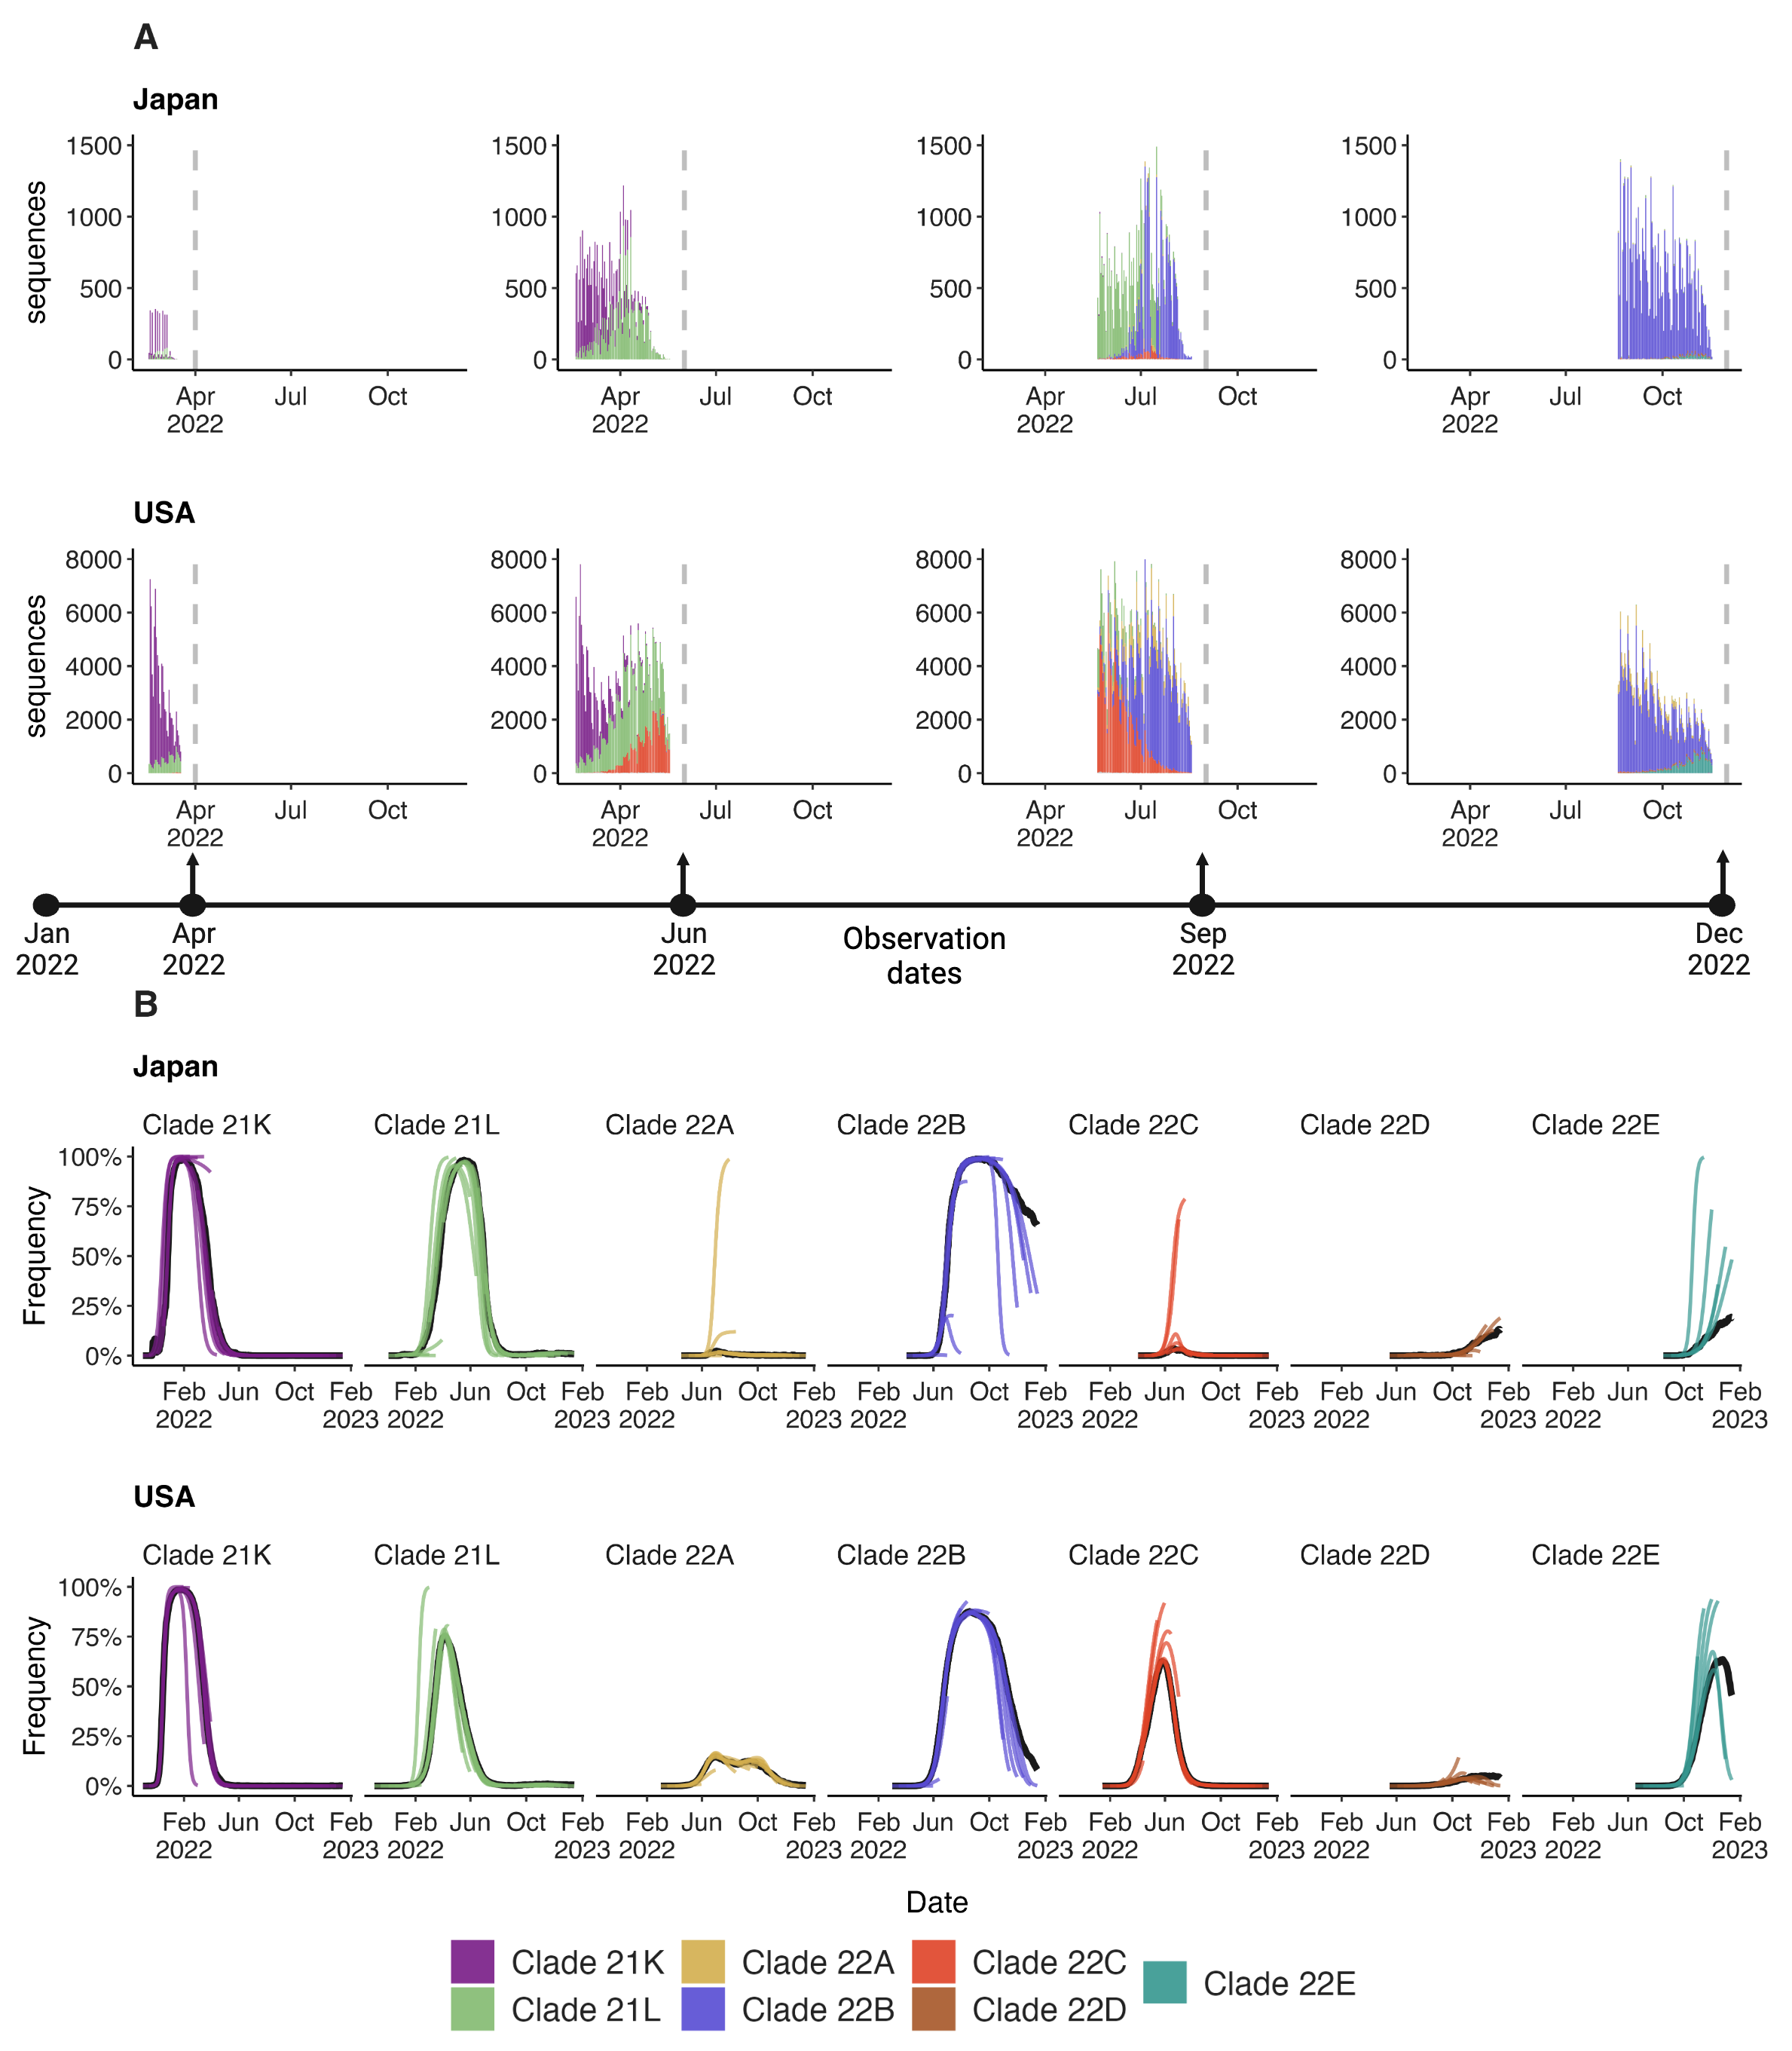
\includegraphics[width=0.8\textwidth=0.01]{figures/Dynamic_est_env.png}
	\caption{\textbf{Example data and predictions for Japan and USA.}
  %MF: I would not say things like "Figure 1 represents". Just jump straight into the discription. 
  %MF: Example text might start with: Nowcasting variant frequencies is complicated by the continuous nature of the data submission process. (A) Variant sequence counts from Japan and United States are shown at 3 different observation dates. Notice ...
	Figure 1 represents a schematic of the dynamic estimation environment.
	Nowcasting variant frequencies is complicated by the continuous nature of the data submission process.
	(A) Variant sequence counts from Japan and United States are shown at 3 different observation dates.
	Notice varying sequence availability at different observation dates. 
	(B) Various frequency nowcasts which depends on the data are shown to vary predictions for different observation dates. 
	}
	\label{LiveNowcasts}
  %MF: Figure filenames and labels we typically want to describe what's in the figure itself since the order is usually subject to change.
\end{figure}


\paragraph{Model Error Comparison}\

We began our comparison by calculating the lag times (difference in days between the date of observation and the date of estimation) as a means of evaluating the performance of the models over time.
This approach provides a reference for understanding how the models perform as the lag time decreases from the forecast period to the nowcast period, where the lag time approaches zero (the date of estimation), specifically from [-30,30].
This enables us to evaluate the effectiveness of the models as we move closer to and further away from the date of observation.

We applied a total of five models for predicting the frequencies of SARS-CoV-2 variants in six countries spanning across different continents (Australia, Brazil, Japan, South Africa, United Kingdom, United States).
The first four models are GARW, FGA, MLR, and Piantham, which are evolutionary forecasting models... %write about whats common
We compare the above 4 models to a naive model to serve as a reference model for comparison.
It is a baseline model which uses simple assumptions to make predictions. %todo mention that this model is worse and that is based on a moving average

The use of multiple models that ranges in complexity allows for a comprehensive evaluation of the performance and robustness of different forecasting methods.
In particular, the use of multiple models allows us to examine if more complex models may be better at capturing epidemiological variant patterns. 

%Mention which models performed best in each lead (no need to mention numbers)
We used our predictions and used several metrics from the framework, specifically Mean Absolute Error (MAE), to assess the relative performance of the models for the six countries (Table~\ref{table1}).
The use of MAE as a metric allows us to quantitatively compare the predictions of different models and determine which model is most accurate in terms of predicting the frequencies of SARS-CoV-2 variants.
The model with the lowest mean MAE error for each country is highlighted as it indicates the best performance among all models (Table~\ref{table1}). 
The results showed that there was a range of values among the models for different leads.
In this analysis, the GARW model performed the best, on average, for -30 and 0 days from the date of estimation.
Notably, for 30 days from the date of estimation, the MLR and GARW models both performed similarly well, with the MLR model exhibiting better performance in Australia, Brazil, and Japan, while the GARW model demonstrated better performance in South Africa, the United Kingdom, and the United States.
These findings indicate that the GARW model exhibited the best performance, as measured by mean absolute error (MAE), among the models evaluated, excluding the naive reference model.
In contrast, the Piantham model performed worst on average among the models tested.

\begin{figure}[H]
	\centering
	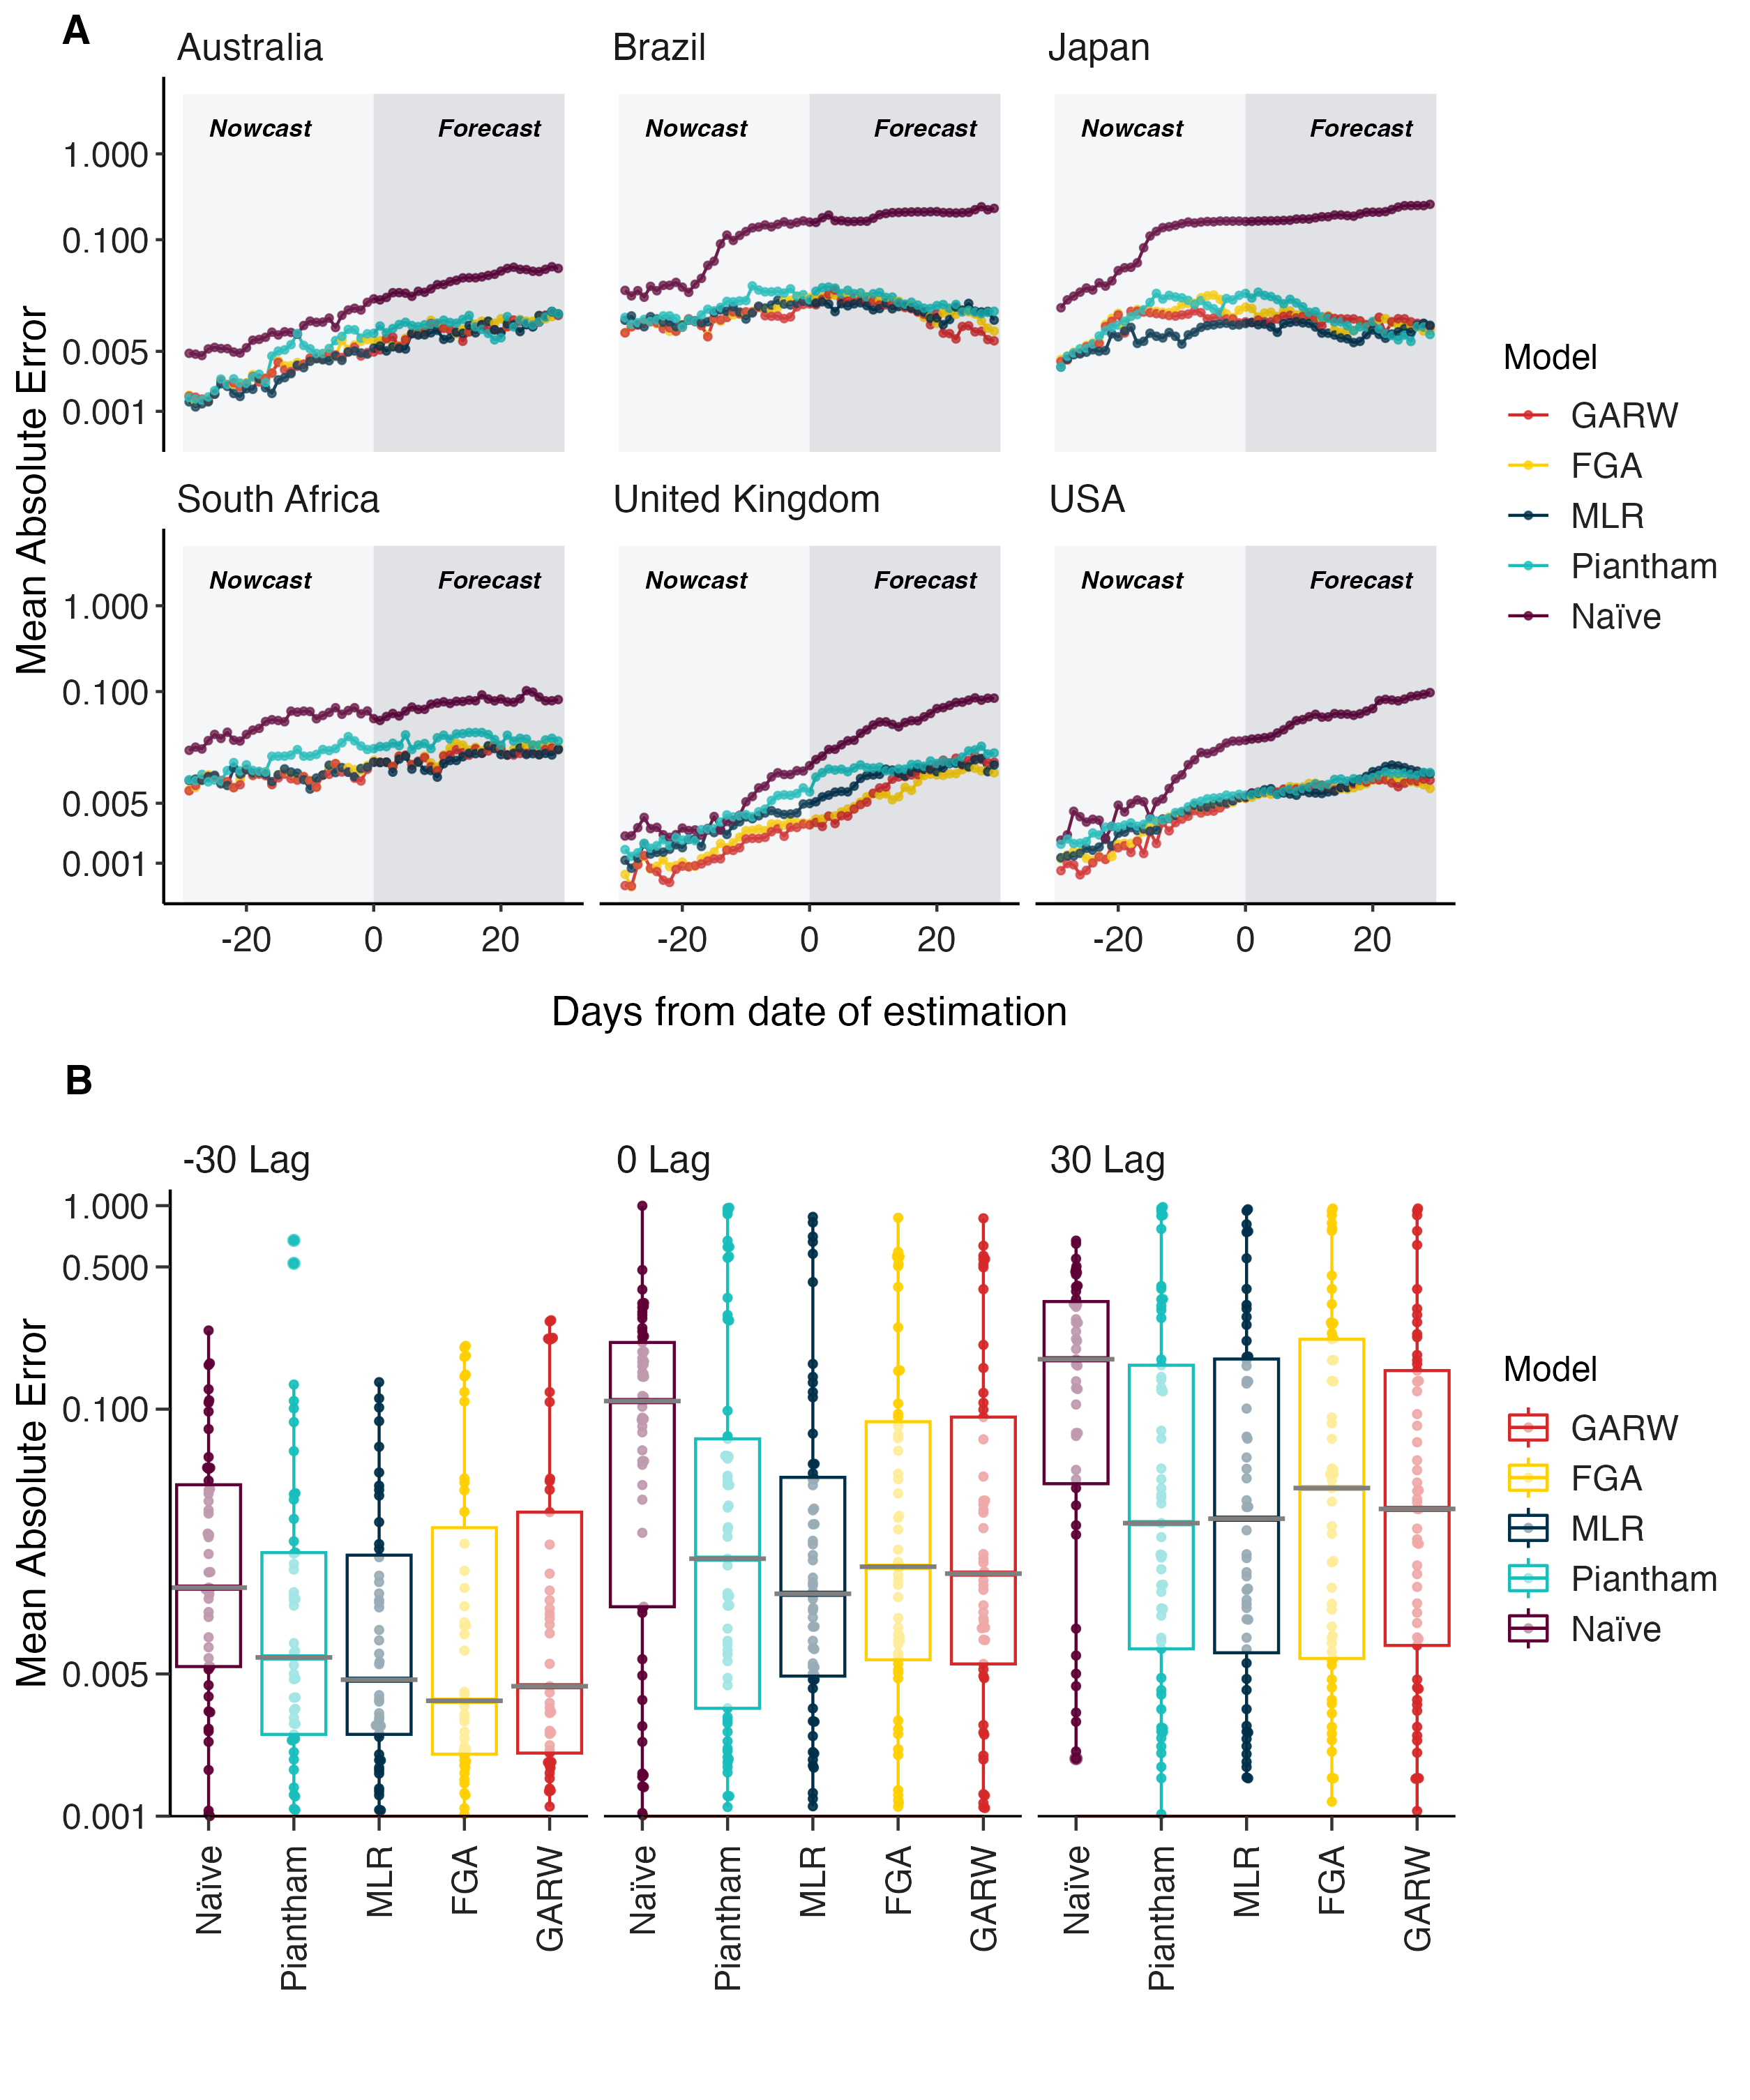
\includegraphics[width=0.8\textwidth]{figures/model_comp.png}
	\caption{\textbf{MAE estimates based on observation date.}
	Figure 2 represents a demonstration of evaluation score (MAE) comparison. 
	(A) comparison of progression of error from nowcasting (-30 days) to forecasting (+30 days) among the five candidate models in six different countries.
	(B) closer look into model performance across three lag times (-30, 0, 30) showing increase in error with farther lag times. 
	}
	\label{Figure 2}
\end{figure}


Models were then compared side by side using error quantiles (25,50, and 75th percentile).
The majority of the models evaluated in this study exhibited median error values within the range of 0 to 10 percent of logarithm of mean absolute error (log(MAE)) (Figure~\ref{Figure 2}.A).
Furthermore, we compared the MAE score distribution between models for all countries (Figure~\ref{Figure 2}.B).
As expected, the results of the analysis show an increase in MAE error for all models as lag or day from estimation increases. 
In other words, as forecasting step increases, the prediction accuracy for all models decreased.

\begin{table}[H]
	\centering
	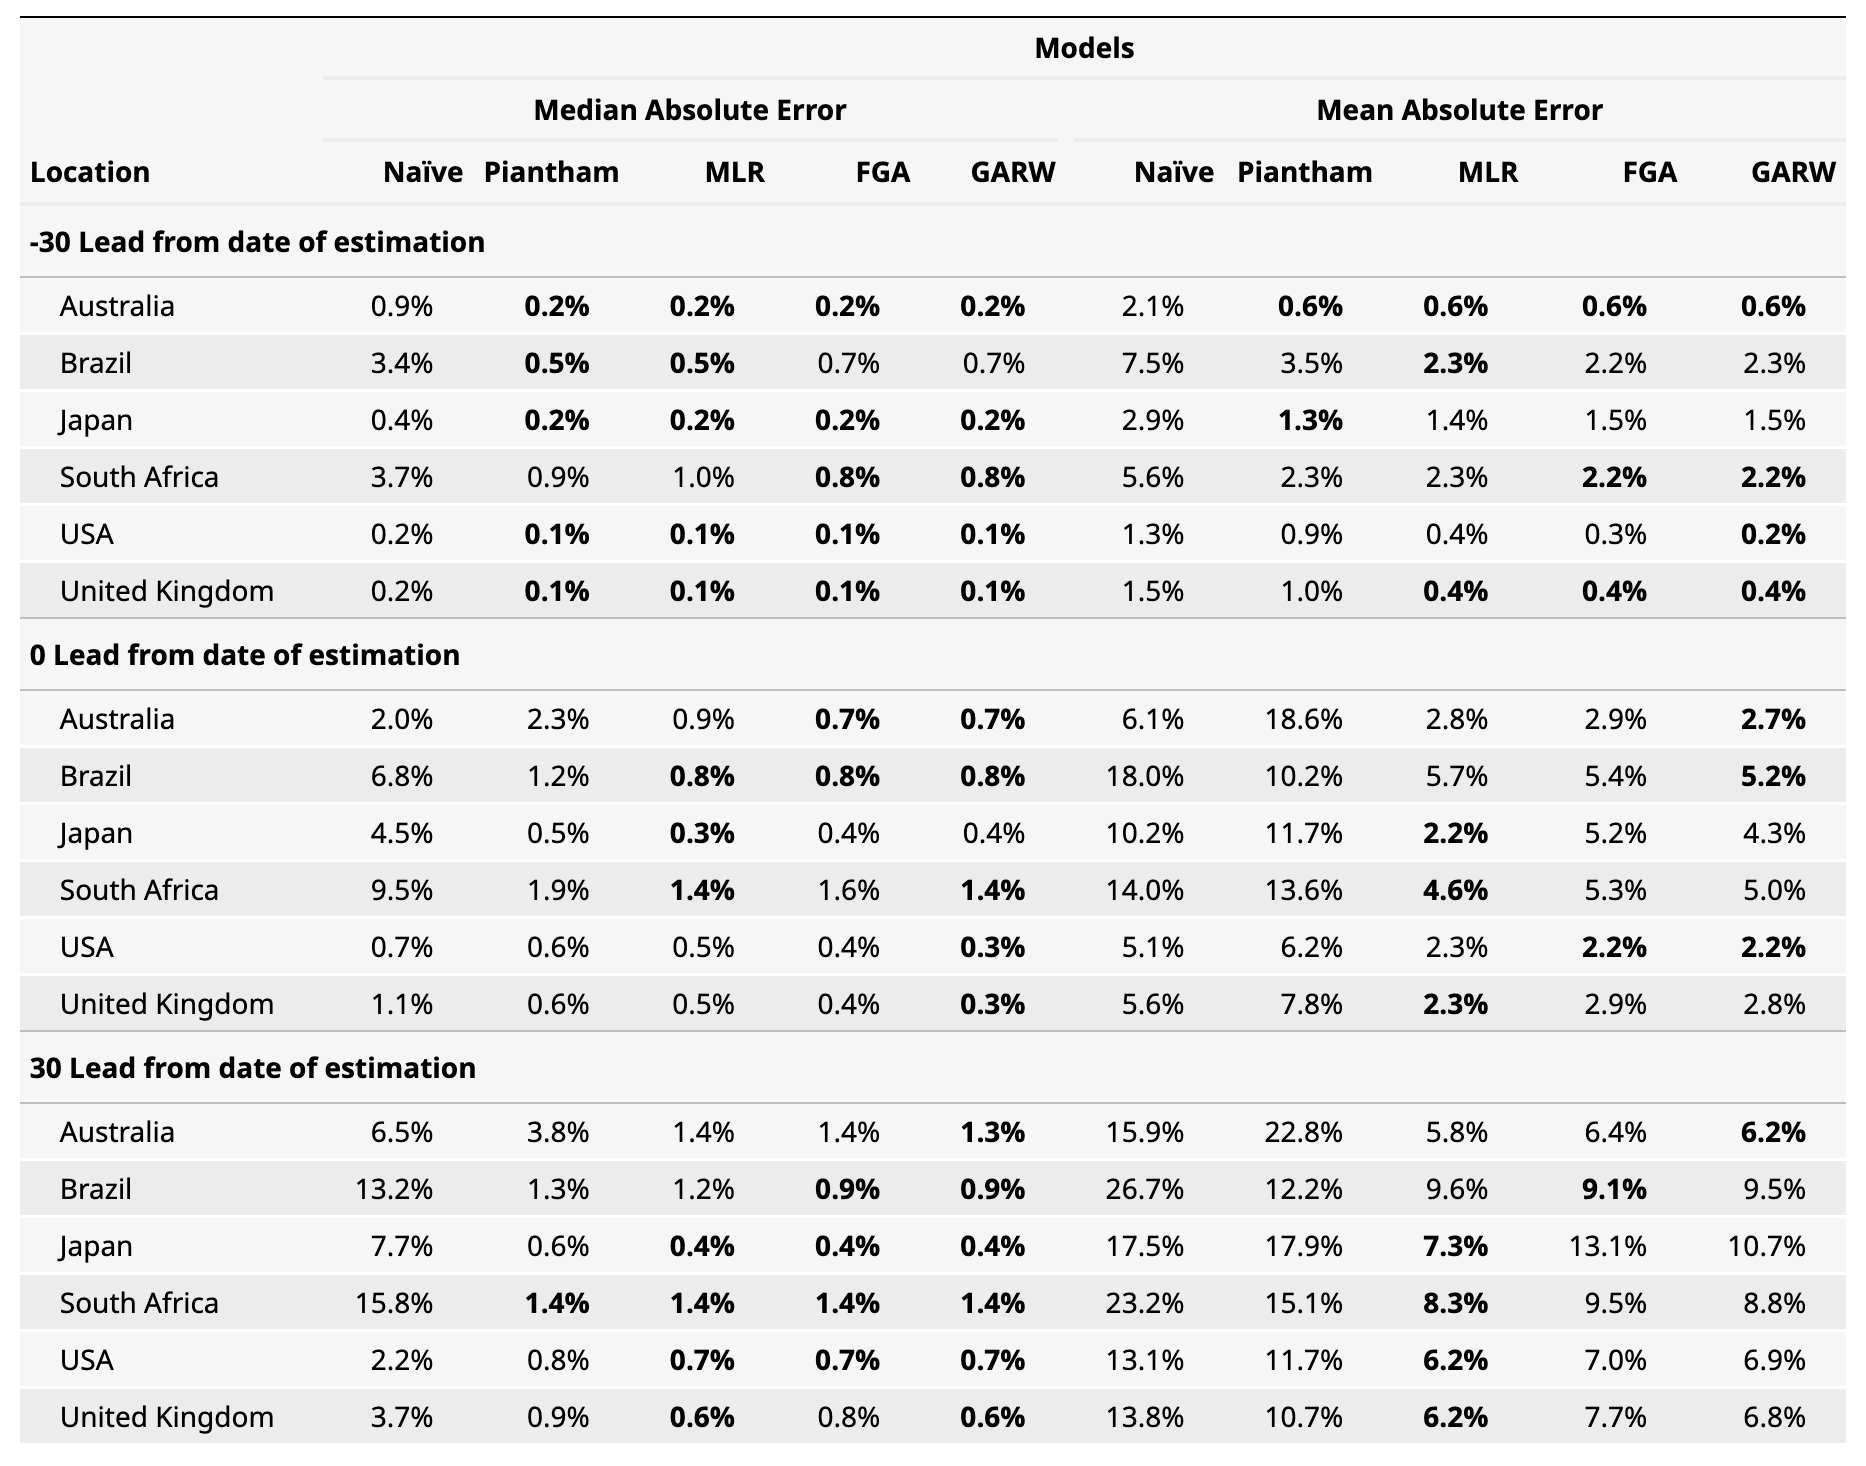
\includegraphics[width=0.6\textwidth]{figures/model_comp_table.png}
	\caption{\textbf{Mean Absolute Error}
	Further legend here.
	}
	\label{table1}
\end{table}

\paragraph{Comparison of Growth Advantages}\

Furthermore, In this study, we investigated the behavior of the growth advantage of different variants in various countries.

Using GARW, MLR, and Piantham models, we standardized the varying growth advantage by estimating the median Growth Advantage values as of that date, we were able to observe when and which variants stabilized in each country (Figure~\ref{Figure 3}). 
The results of the analysis revealed that the majority of countries displayed stabilization with regard to the Omicron 22A, B, and C variants, with the exception of Japan.
This discrepancy may be attributed to Japan's limited availability of sequence data or other imperfections in the data.
%they mostly stabilized except Japan % and why (motivated us to next step of analysis)

\begin{figure}[H]
	\centering
    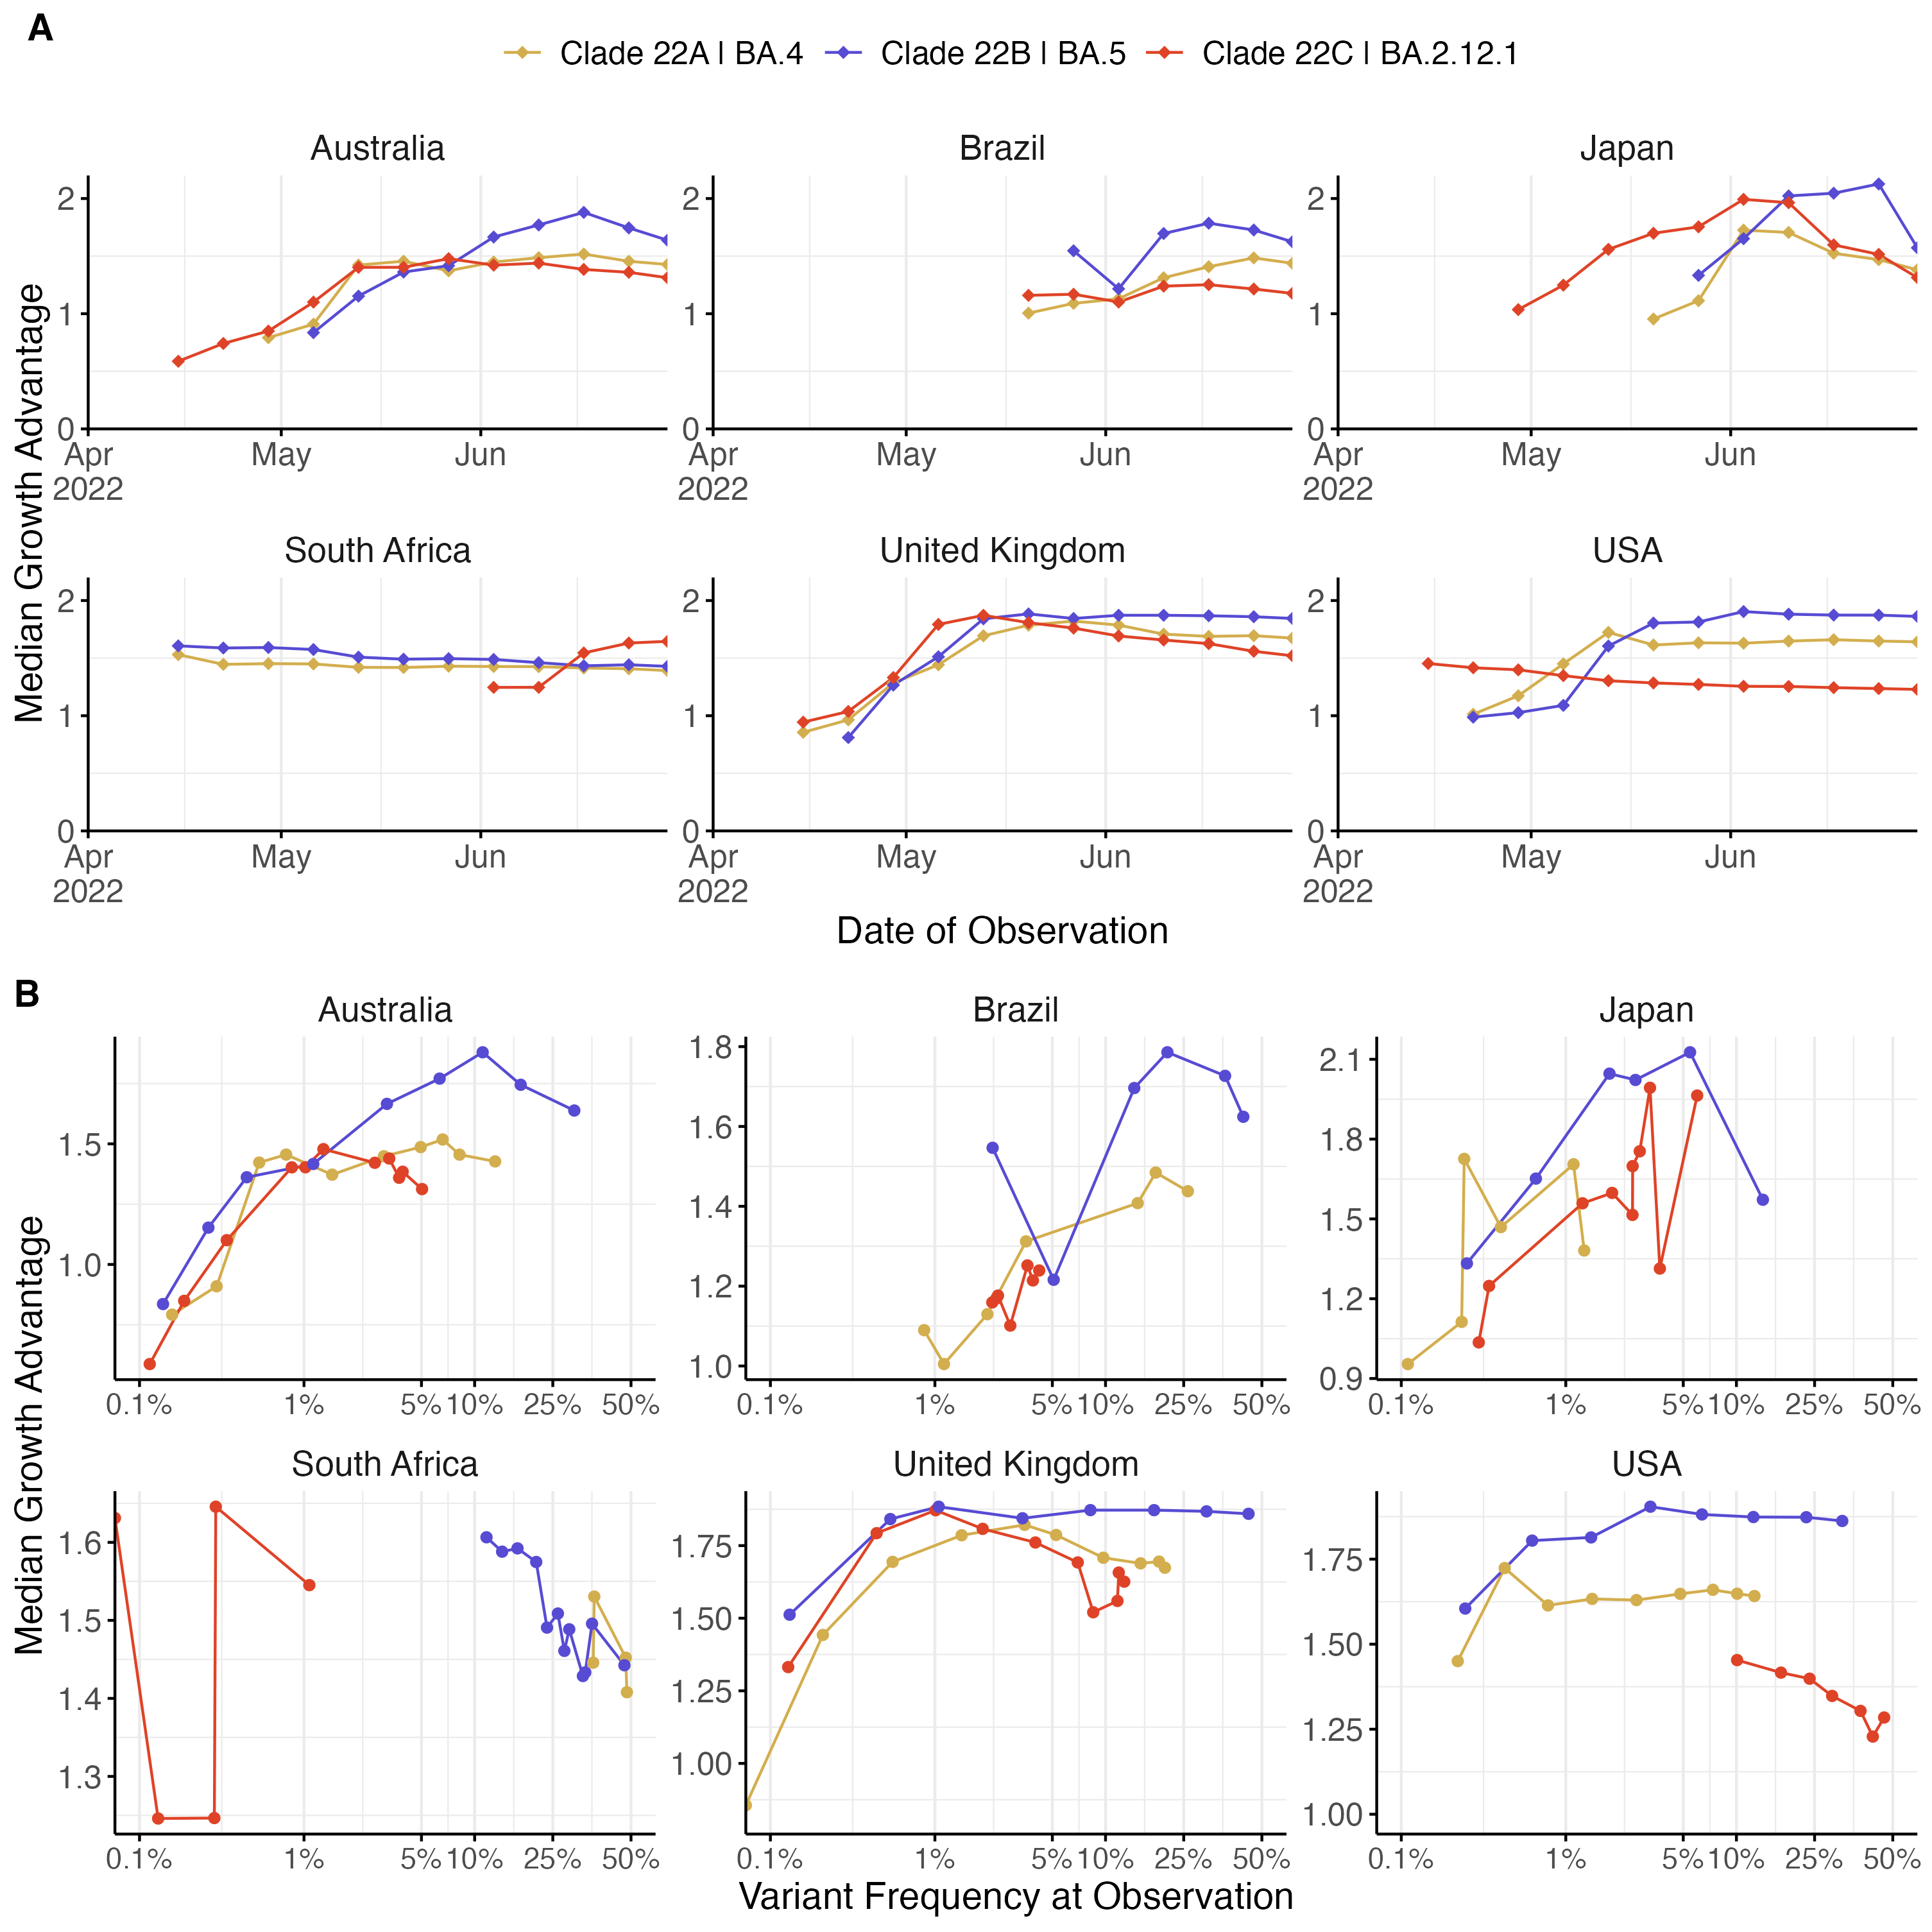
\includegraphics[width=1.1\textwidth]{figures/ga_estimates.png}
	\caption{\textbf{Growth Advantage of variants over time}
	Figure 3 demonstrates the stabilization of growth advantage of different clades relative to BA.1.
	(A) Differences among growth advantages among three clades in six different countries. 
	Noticing how quickly variants dial and stabilize between different countries.
	(B) Observation of stabilization of growth advantages according to the percent of variant frequency at observation.
	}
	\label{Figure 3}
\end{figure}

\paragraph{Inferential Regression Model}\

TODO

\paragraph{Variation in frequency error}\

In order to investigate the variability among different countries and models and explain the emergence of error patterns in the forecasts, we employed a step-wise regression model to identify various variables that may contribute to errors in mean absolute error (MAE) of the models.
These variables were variants selective pressure, lead, sequence availability, fraction of sequences available within a week, median delay of data submission. 
Subsequently, a multivariate regression model was constructed to predict MAE errors, which was then fitted to SARS-CoV-2 variant data for all countries, as well as for each country individually.

\textbf{Model Specification}

maybe stepwise regression??

All countries model with logit transformation?

Model with interactions?

Mixture model?


Maybe just use correlations between the variables that we believe has an association?


log(MAE = xxxx)


\textbf{Model Performance}

R2 for each country (maybe make a table)
R2 for full model with all countries

Confidence intervals
prediction interval


%we built a linear model
% we picked these variables to predict the error
%identified which variables are of most importance
% 


%%% DISCUSSION %%%
\section*{Discussion}

% Interpretation of the results

%Main findings

%Introducing the discussion

By developing a framework for comparing models of SARS-CoV-2 variant frequency and their forecasts, we find that most models of variant frequency perform well and are able to produce reasonable forecasts.
However, we find that naive models such as a 7-day moving average may not perform well due to the live nature of sequencing efforts e.g. delays between collection and availability of new samples.
Overall, [insert fact here] it appears that differences in model accuracy can be attributed to differences in the surveillance and sequencing efforts themselves.

Consistent with most time series models, we find an increase in model errors and their variance as estimates go farther in the future from the observation date.
These long-term forecasts also appear to have heavier tails which indicate increase in extreme values and may be attributable to model break down or the emergence of new variants.  

% Through our present framework, we modeled SARS-CoV-2 variant frequencies which allowed us to estimate transmission differences between clades.
% From our initial examination of the data we find that sequencing data exhibit temporal and geographical variation such that data vary based on the date of observation. 
% Furthermore, we find that the six countries examined show varying ranges of back-filling of data, submission delays, and missing data. 
%
% %patterns of error observed from analysis
% Taking a closer look into the errors generated by our models, we find that there is a consistent patterns of errors (Mean Absolute Error) observed among the different models examined that lend themselves to different interpretation. 

%Brazil and japan and south africa? breaking? we wanna see why they break??
%Something may be wrong with them > next analysis?


% Our findings suggest that the variations in error patterns observed are likely attributable to the way in which the models handle data issues across different countries. 
As such inferences from forecasting models with underlying poor sequencing efforts may not be a reliable approach for such instances without a more contextual understanding of the limitations.
Additionally, standard modeling practices involve presenting the frequency of variants from 30 days prior as the "truth" (Reference? using outbreak.info?); however, our analysis of the naive model reveals a substantial discrepancy between the naive frequencies and the retrospective truth for all countries, except for the US and UK, where a rigorous sequencing effort is in place. 
Importantly, we find that our multinomial logistic regression model (MLR) demonstrates a tangible improvement in accuracy for Australia, Brazil, Japan, and South Africa.

%Trevors point about naive model that last 30 days is not actually truth
%Japan: Cornelius > It could be that they have a lot of bunching/overdispersion due to the way labs upload, e.g. one day it’s all North, other day all South etc.

From our analysis of transmission dynamics, we find that it takes a shorter amount of time for different variant clades to stabilizer in countries with more robust sequencing efforts. 
Our analysis also suggest that the variability between different countries' growth advantage estimates for different clades may not necessarily be biological but due to data limitations that we show here.
To understand why different countries dial in quicker, We find that at higher frequencies the growth advantage estimates for the clades begin to stabilize. 
%temporal resolution is also important here, why at lower freq US and UK are still doing good

* these errors affect growth advantage estimates  (figure 3)
* different variant dynamics happening in different countries which explain why some countries (SA)
* point about frequency needed for good estimates
* from investigating variables of interest (which quantify sequencing efforts) we saw that it plays a role in explaining the variation in error
* Non sequencing heterogeneity may also explain error

%Limitations

%Future research

%%% METHODS %%%
\section*{Methods}

\paragraph{Preparing sequence counts and case counts}

We prepare sequence count datasets in order to mirror a live nowcasting environment. 
For a given pivot or observation date, we filter to all sequences which were collected 90 days before the observation date. 
In order to properly account for submission delays in this collection process, we additionally filter to those sequences which were submitted before the observation day.
These sequences are then counted according to their Nextstrain clade assignment to produce sequence counts for each Nextstrain clade each day over the period of interest. 
These sequence counts are produced independent for … countries including Australia, Brazil, Japan, the United States, the United Kingdom, and South Africa.
We repeat this process for a series of observations days which are every 7 days starting with … and ending with … giving a total of … datasets for each country.
Since two models (FGA and GARW) also use case counts for their estimates, we additionally prepare data sets using case counts over the time periods of interest as available from Our World in Data.

\paragraph{Frequency dynamics and transmission advantages}%

We implement and evaluate several models of variant frequencies.
Each of these methods estimate variant frequencies over time and as well as estimate the transmission advantage of given variant relative to a baseline variant $R_{t}^{v} / R_{t}^{u}$.

The 4 models of interest are: Multinomial Logistic Regression (MLR), Piantham model (cite), a fixed growth advantage model (FGA), and a growth advantage random walk model (GARW). 
Details for each of these models can be found in the corresponding citations above.

We provide a brief mathematical overview of these methods below.

The models mentioned above estimate the frequency  $f_{v}(t)$ of variant $v$ at time $t$ using sequence counts and/or case counts of the form described in the previous section.
All models simultaneously estimate the variant transmission advantages $\Delta_{v} = \frac{R_{t}^{v}}{R_{t}^{\text{pivot}}}$ where $R_{t}^{v}$ is the effective reproduction number for variant $v$.
We can interpret these transmission advantages as the relative effective reproduction number of a variant against a given pivot variant.
Growth advantages presented in this manuscript are relative to the baseline Omicron 21L (BA.1) strain, providing a point of reference for competing growth advantages and how median values change over time. 
The models differ in assumptions in computing this quantity i.e. MLR depends on an assumption of a fixed generation time, Piantham assumes the total prevalence is fixed in time, while GARW / FGA additionally model the transmission process using case count data.
Further details on the model formats can be found in their respective citations.
All models were implemented using the evofr (evolutionary forecasting) software package in Python using Numpyro for inference.
We compare the four models to a naive model which is implemented as a 7-day moving average on the retrospective raw frequencies.

% * Framework
%
% In our efforts to investigate how modeling approaches handle data issues, we developed a novel framework for standardizing and accurately estimating real-time nowcast and forecast targets, and to facilitate comparisons of forecasting and nowcasting accuracy between various statistical models.
% This framework utilizes live surveillance data to examine the empirical aspects of evolutionary forecasting by forecasting targets which includes viral pathogen frequencies, pathogen growth advantages, and incidence estimates. 
% Additionally, the framework provides a statistical scoring rule system for evaluating the effectiveness of different modeling approaches.
% The purpose of this study is to investigate the utility of this framework in the context of evolutionary forecasting and to improve our understanding of the factors that influence the accuracy of nowcast and forecast targets.


\paragraph{Evaluation Criteria}

We evaluate the error between the model predicted frequencies and the truth set averaged across each variant at a given time point using three metrics: root mean squared error (RMSE), mean absolute error (MAE), and a multinomial log-likelihood.

\paragraph{Generating predictors of error}

We explore four key variables to better encompass the effect of sequencing efforts which are fraction of sequences available, sequences available, median delay and lead. 
These variables are defined as fraction of sequences available within 14 days of the prediction time, total sequences availability within 14 days of the prediction time, median delay of sequence submission, and lead time from prediction day subsequently for each location (Figure~\ref{Figure 4}).
To calculate these variables, we selected a 14-day window of data before each and every observation date and used the collection and submission dates to determine their availability in addition to the period of discrepancy between the collection and submission for each country.
All variables were calculated using Rstudio statistical software.

\begin{figure}[H]
	\centering
    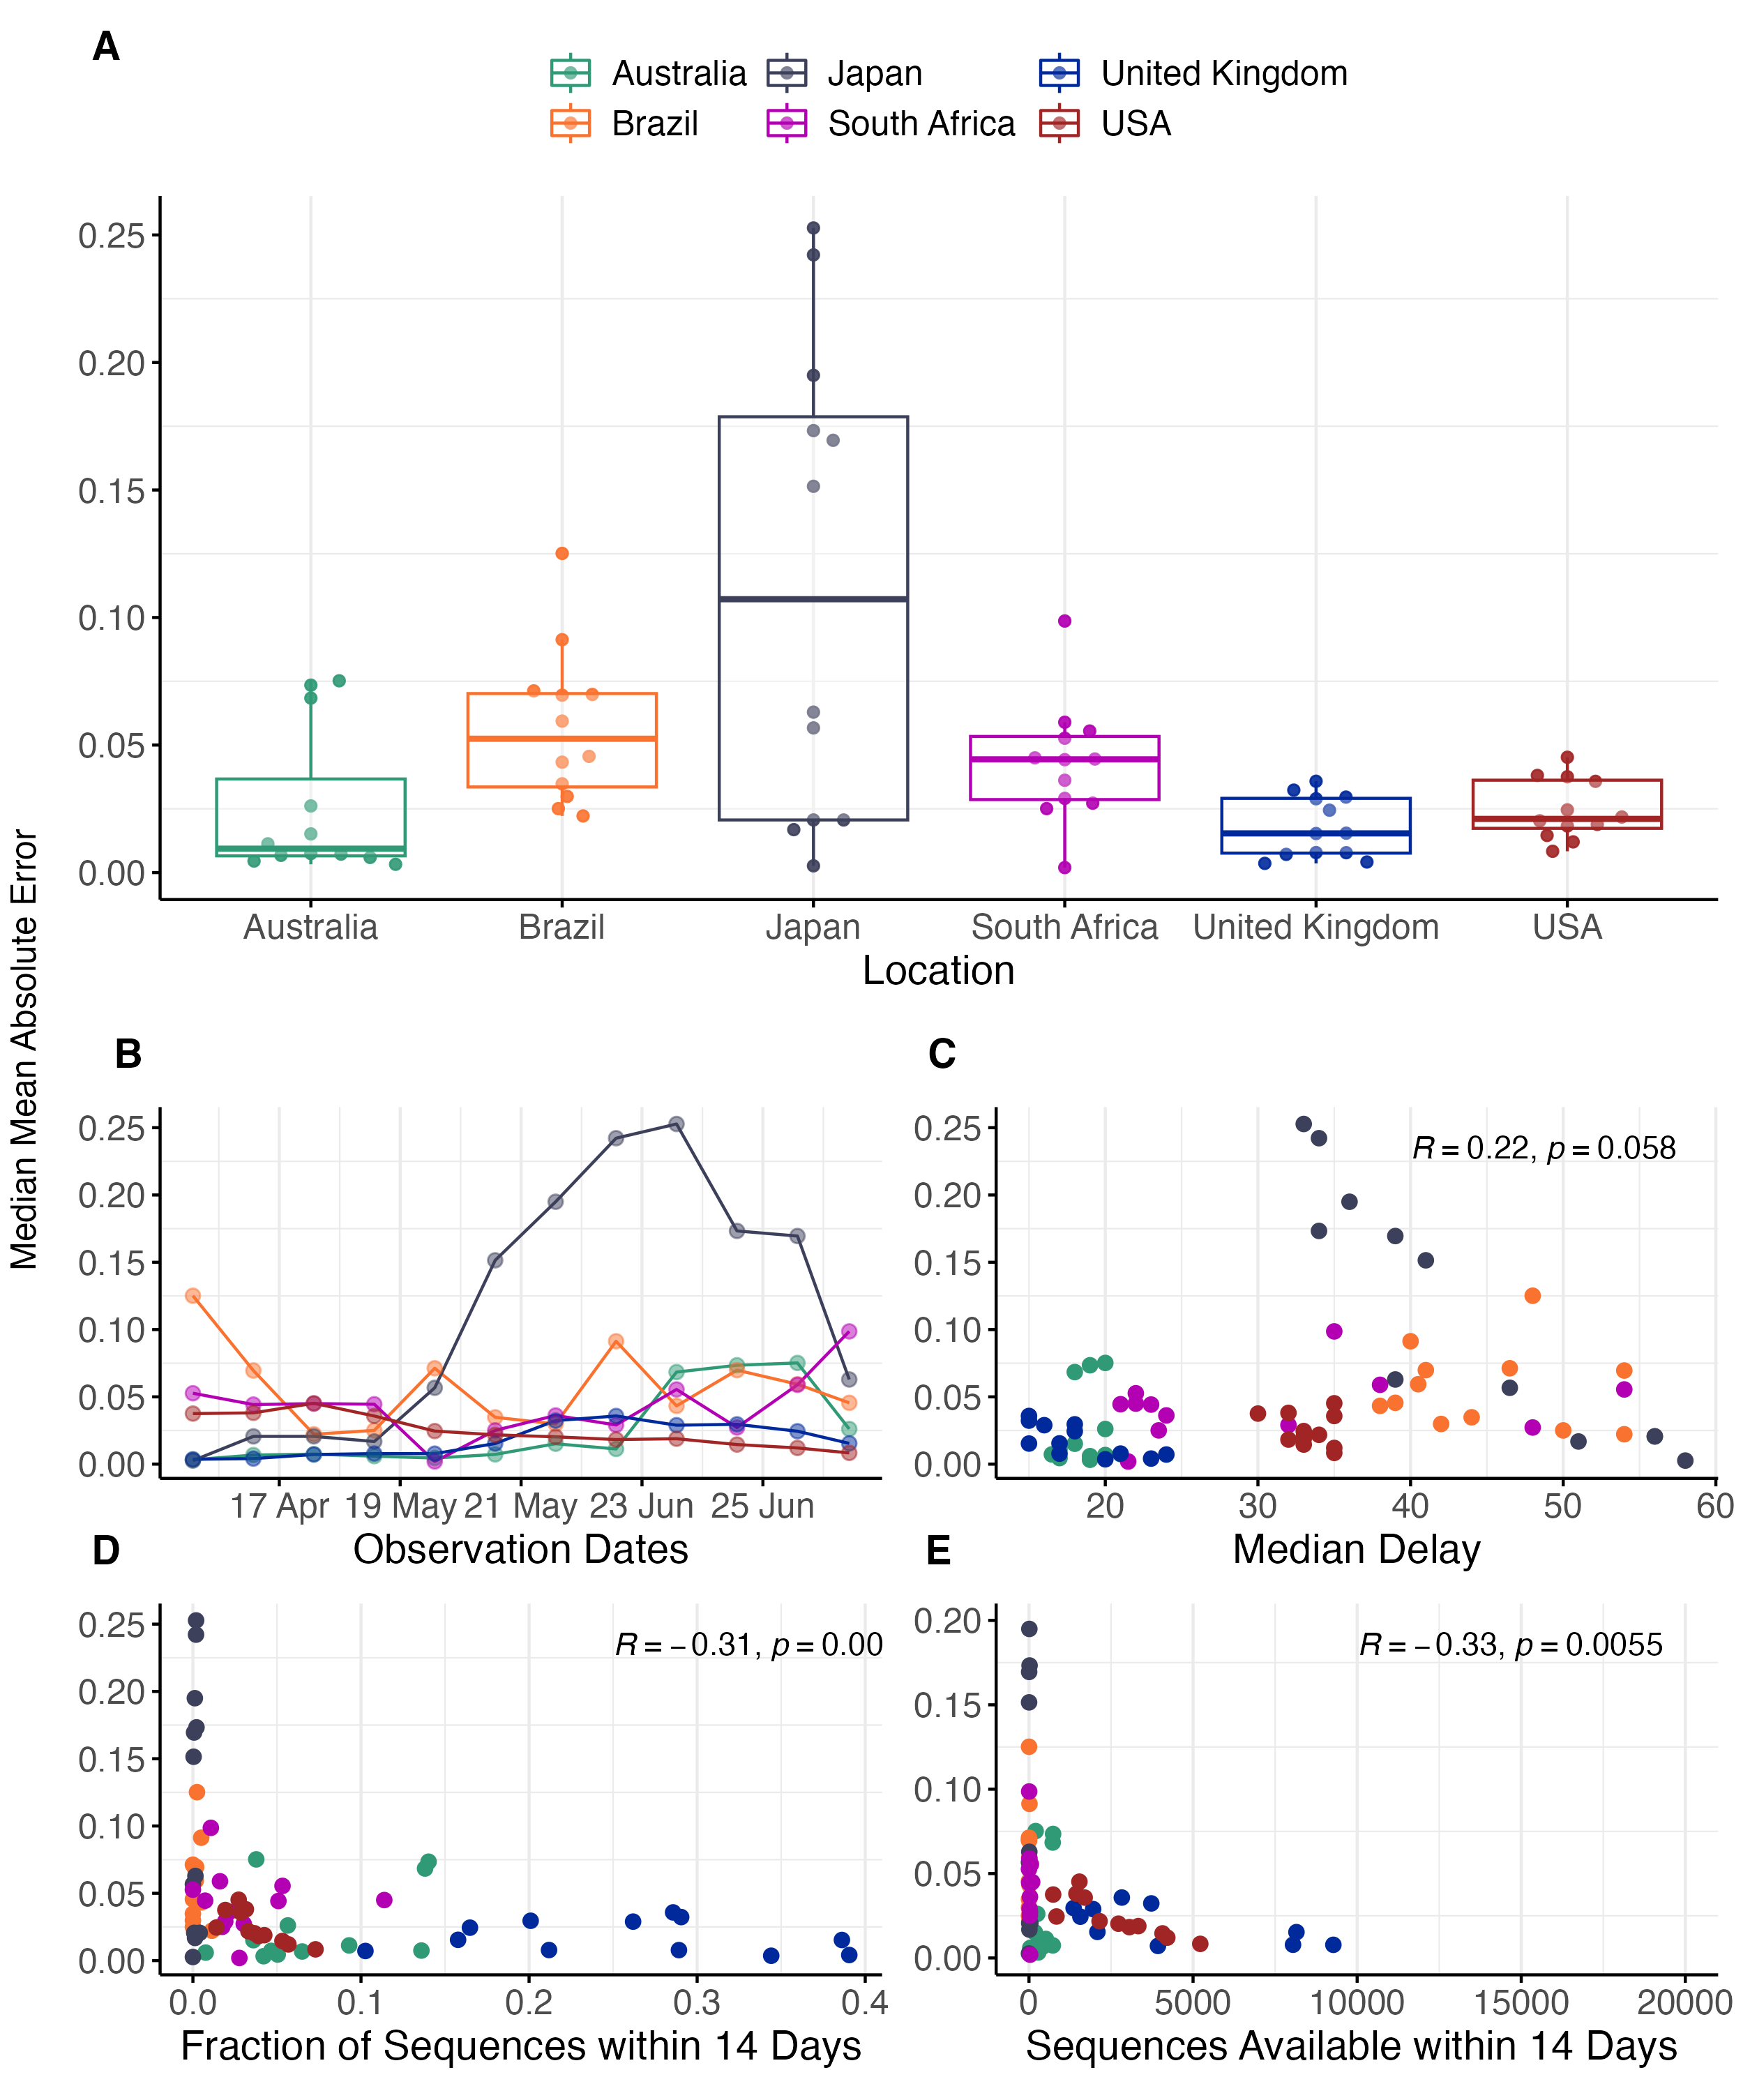
\includegraphics[width=1.1\textwidth]{figures/Var_of_interest.png}
	\caption{\textbf{Variables of interest in predicting forecasting error}
	Further legend here.
	}
	\label{Figure 4}
\end{figure}


\paragraph{Regression analyses}

%TODO: Give details on how we transform the data in the various regression analyses and in plots

%How to replicate the different analyses
%Talking about what variables mean

\section*{Data and code accessibility}

Sequence data including date and location of collection as well as clade annotation was obtained via the Nextstrain-curated
dataset that pulls data from GISAID database. 


Derived data of sequence counts and case counts, along with all source code used to analyze
this data and produce figures is available via the GitHub repository https://github.com/blab/ncov-forecasting-fit


%%% REFERENCES %%%
\bibliographystyle{plos}
\bibliography{ncov-forecasting-fit}

\end{document}
